\documentclass[11pt]{article}
% Shared preamble for the hanzo-kernel Paper 07 series.
% One style, one vocabulary, inputted by every paper so the series reads as one voice.
\usepackage[margin=1in]{geometry}
\usepackage{booktabs}
\usepackage{amsmath}
\usepackage{amssymb}
\usepackage{graphicx}
\usepackage{xcolor}
\usepackage{hyperref}
\hypersetup{colorlinks=true, linkcolor=blue, urlcolor=blue, citecolor=blue}
\usepackage{enumitem}
\usepackage{listings}
\usepackage{array}

\definecolor{kw}{rgb}{0.13,0.29,0.53}
\definecolor{cmt}{rgb}{0.40,0.40,0.40}
\definecolor{str}{rgb}{0.16,0.50,0.16}
\lstset{
  basicstyle=\ttfamily\footnotesize,
  keywordstyle=\color{kw}\bfseries,
  commentstyle=\color{cmt}\itshape,
  stringstyle=\color{str},
  showstringspaces=false,
  breaklines=true,
  columns=fullflexible,
  frame=single,
  framesep=4pt,
}
\lstdefinelanguage{Rust}{
  morekeywords={fn,let,mut,pub,struct,impl,trait,enum,match,if,else,for,while,loop,return,use,mod,crate,self,super,async,await,where,type,const,static,unsafe,ref,move,dyn,as,true,false},
  morecomment=[l]{//}, morecomment=[s]{/*}{*/}, morestring=[b]", sensitive=true,
}

\newcommand{\x}{\ensuremath{\times}}
\newcommand{\dpa}{\texttt{dp4a}}
\newcommand{\hk}{\texttt{hanzo-kernel}}
\newcommand{\code}[1]{\texttt{#1}}

% Absorb minor prose overfulls without rivers; keep line-breaking sane.
\tolerance=800
\emergencystretch=3em

\usepackage{pgfplots}
\pgfplotsset{compat=1.16}

\newcommand{\Tring}{\ensuremath{T_{\mathrm{ring}}}}
\newcommand{\dmodel}{\ensuremath{d_{\mathrm{model}}}}
\newcommand{\Gam}{\ensuremath{\Gamma}}

\title{\textbf{The Latency Physics of Geo-Distributed\\ Autoregressive Decode}}
\author{Hanzo AI --- ML Systems}
\date{An analytical systems paper --- companion to the cross-backend inference measurements}

\begin{document}
\maketitle

\begin{abstract}
Splitting a large language model across machines that sit far apart is often imagined as
``BitTorrent for AI'': pool everyone's memory and the model runs. For \emph{loading} weights and
for \emph{batched throughput} that intuition is right. For \emph{single-stream, interactive decode}
it is exactly wrong, and this paper derives why. We separate the two costs of a node boundary.
\textbf{Bandwidth is trivial}: the only tensor that crosses a pipeline boundary is the hidden state
for the in-flight tokens, \dmodel${}\times n_{\mathrm{tok}}\times b$ bytes --- $\sim$32\,KiB for one
token of a 700B-class model --- which serializes in $\approx$0.1\,ms over our measured 280\,MB/s
wired mesh, and the KV cache never crosses at all. \textbf{Latency is the wall}: autoregressive
decode is a strict dependency chain, so each generated token must traverse every node once, and the
next token cannot begin until the current one returns. Per-token decode rate is therefore
$r=1/(C+\Tring)$, where $C$ is the summed compute and $\Tring=\sum_i \ell_i$ is the one-way latency
of a full loop around the ring. Because \Tring{} adds to a per-token denominator, a geo-distributed
ring (Hong Kong\,$\to$\,Dublin\,$\to$\,New York, $\Tring\!\approx\!280$\,ms) floors single-stream
decode at $\approx$3\,tok/s \emph{regardless of GPU speed} --- the wall is the speed of light in
fiber, not the accelerator. The headline result is the cure: \textbf{speculative decoding converts
$K$ sequential network traversals into one}. A local draft model proposes $K$ tokens at full LAN
speed; the distributed model verifies all $K$ in a single pipeline pass; at acceptance rate $\alpha$
the effective rate is $r_{\mathrm{spec}}=\frac{1-\alpha^{K+1}}{1-\alpha}\big/(Kc_d+C+\Tring)$, which
recovers 12--21\,tok/s on the same 280\,ms ring --- interactive speeds from an intercontinental
deployment. We close with four placement laws, including a derivation that pipeline parallelism
($O(\text{nodes})$ hops/token) strictly dominates tensor parallelism ($O(\text{layers})$
all-reduces/token) over any slow link by a factor of $\sim\!4L/N$. Every model here is analytical
and labelled as such; the one measured number is the 280\,MB/s link.
\end{abstract}

\section{Two regimes: dependency-bound vs.\ throughput-bound}
\label{sec:dichotomy}

The whole paper turns on one distinction, so we state it first.

A computation is \textbf{throughput-bound} when its pieces are independent: they can be done in any
order, in parallel, and the only thing that matters is aggregate bytes-or-flops per second. Network
\emph{latency} barely touches such a workload --- a slow link means each piece arrives a little
later, but no piece waits on another, so the pipe stays full and throughput is set by
\emph{bandwidth}. Downloading a file is the canonical case; so is a batch of a thousand independent
inference requests.

A computation is \textbf{dependency-bound} when its pieces form a chain: piece $t+1$ cannot start
until piece $t$ finishes. Now latency is on the critical path of \emph{every} step and cannot be
hidden, because there is no independent work to overlap it with. Bandwidth is almost irrelevant ---
the messages are tiny --- and the wall is the round-trip time.

Autoregressive decode is the purest dependency chain in production machine learning. Token $t+1$ is
sampled from the model's output after token $t$ has been fed back as input; \emph{within} a token,
layer $\ell+1$ consumes the output of layer $\ell$. There is exactly one token in flight for a
single stream, so there is nothing to overlap. Distributing that chain across nodes does not add
parallelism to a single stream --- it adds hops to the chain. This is why the ``pool everyone's
GPUs'' picture, which is a throughput picture, gives the wrong answer for interactive decode, which
is a dependency problem. The rest of the paper makes both halves quantitative.

\paragraph{Parameters and provenance.}
Table~\ref{tab:params} lists the symbols and the reference values used in the worked numbers.
\emph{One} value is measured --- the 280\,MB/s link goodput, from iperf3 on our direct 2.5\,GbE
mesh. The representative one-way fiber latencies are physical (Section~\ref{sec:wall}) and are not
our measurements; the model geometry (\dmodel, $L$) is that of a public 700B-class dense/MoE model;
the local decode ceiling $r_0$ and draft rate $r_d$ are stated parameters, not claims about a
specific box. Every rate, table, and plot downstream is a closed-form evaluation of the models in
this paper, not an experiment.

\begin{table}[h]
\centering
\small
\caption{Symbols and reference values. Only $W$ is measured.}
\label{tab:params}
\begin{tabular}{l l l l}
\toprule
Symbol & Meaning & Reference value & Provenance\\
\midrule
$N$        & pipeline nodes (stages)                 & 3                 & scenario\\
$L$        & transformer layers                      & $\sim$100         & 700B-class model\\
\dmodel    & hidden size                             & 16384             & 700B-class model\\
$b$        & activation bytes/element (bf16)         & 2                 & format\\
$W$        & per-link goodput                        & \textbf{280\,MB/s} & \textbf{measured (2.5\,GbE)}\\
$\ell_i$   & one-way latency of hop $i$              & 40--130\,ms (geo) & physical (fiber)\\
$\Tring$   & ring latency $\sum_{i=1}^N \ell_i$      & 280\,ms (geo)     & physical (fiber)\\
$C=1/r_0$  & target compute per decode step          & 33\,ms ($r_0{=}30$) & parameter\\
$c_d=1/r_d$& local draft time per token              & 5\,ms ($r_d{=}200$) & parameter\\
$\alpha$   & speculative acceptance rate             & 0.6--0.9          & parameter\\
$K$        & draft length (tokens/round)             & 1--24             & swept\\
\bottomrule
\end{tabular}
\end{table}

\section{The crossing tensor: bandwidth is trivial}
\label{sec:bandwidth}

In pipeline parallelism (PP) the model is partitioned by \emph{layer}: node $i$ owns a contiguous
stack of $L/N$ layers. The only data that crosses the boundary between node $i$ and node $i{+}1$ is
the residual-stream hidden state at that layer cut --- one activation tensor of shape
$[\,n_{\mathrm{tok}},\ \dmodel\,]$ in the activation dtype. Its size is
\begin{equation}
B_{\mathrm{hop}} \;=\; n_{\mathrm{tok}}\cdot \dmodel \cdot b \quad\text{bytes},
\label{eq:bhop}
\end{equation}
and the time to push it across a link of goodput $W$ is $t_{\mathrm{xmit}}=B_{\mathrm{hop}}/W$.
Three properties of Eq.~\eqref{eq:bhop} decide the paper.

\paragraph{It is independent of model depth.} $B_{\mathrm{hop}}$ contains no $L$. Only the
\emph{width} \dmodel{} and the number of in-flight tokens appear, because exactly one activation
crosses each cut no matter how many layers sit behind it. A deeper model costs more
\emph{compute} per node but not more \emph{bytes} per hop. This is the structural reason PP is the
right WAN topology (Section~\ref{sec:pptp}).

\paragraph{The KV cache never crosses the wire.} Each node holds the keys and values for
\emph{its own} layers and reuses them locally on every step. The KV cache is the large, context-
growing state; it stays put. What crosses is only the small, fixed-size residual vector. Distributing
the model does not distribute the KV traffic --- there is none across the boundary.

\paragraph{For decode it is a rounding error.} For a single decoded token, $n_{\mathrm{tok}}=1$.
With the 700B-class width $\dmodel=16384$ and bf16 ($b=2$),
\[
B_{\mathrm{hop}} = 1\cdot 16384 \cdot 2 = 32{,}768~\text{bytes} = 32~\text{KiB},
\qquad
t_{\mathrm{xmit}} = \frac{32{,}768}{280\times10^6} \approx 0.117~\text{ms}
\]
over our \emph{measured} 280\,MB/s mesh. Even at a serving-scale aggregate of 1000\,tok/s each hop
carries $\sim$32\,MB/s --- about a tenth of a single 2.5\,GbE link, and nothing on a datacenter WAN.
\textbf{Bandwidth is never the constraint for decode.} (It can matter for large-prompt prefill,
where $n_{\mathrm{tok}}=P$: a 2000-token prompt crosses 65.5\,MB per hop, $\approx$234\,ms to
serialize over 280\,MB/s --- but that is a bulk, streamable, latency-insensitive transfer that a
fatter pipe fixes. It is a throughput cost, not a wall; Section~\ref{sec:regimes}.)

\section{The wall: latency floors single-stream decode}
\label{sec:wall}

Now the cost that does not go away. Generating one token drives the hidden state through all $N$
nodes in sequence: node~1 embeds and runs its layers, hands off to node~2, and so on to node~$N$,
which produces the final hidden state; the model head samples the next token, which must return to
node~1 to begin the next step. Counting hops on the critical path: $N-1$ forward hand-offs plus one
\emph{return} hop that closes the loop, i.e.\ $N$ inter-node latencies per token. Writing $\ell_i$
for the one-way latency of hop $i$ and $c_i$ for node $i$'s compute on its layer slice,
\begin{equation}
T_{\mathrm{tok}} \;=\; \underbrace{\sum_{i=1}^{N} c_i}_{\textstyle C}
\;+\; \underbrace{\sum_{i=1}^{N} \ell_i}_{\textstyle \Tring},
\qquad
r \;=\; \frac{1}{T_{\mathrm{tok}}} \;=\; \frac{1}{C + \Tring}.
\label{eq:wall}
\end{equation}
Two facts about Eq.~\eqref{eq:wall} carry the argument.

\paragraph{PP gives a single stream zero compute speedup --- only added latency.} For one in-flight
token, only one node computes at a time; the other $N-1$ idle (the pipeline is empty). So the total
compute $C=\sum_i c_i$ equals the monolithic single-node decode compute; splitting the model does
not make one stream's arithmetic faster. What splitting \emph{adds} is $\Tring$. PP buys memory
capacity (a 700B model that fits nowhere else) and, with batching, throughput
(Section~\ref{sec:regimes}) --- never single-stream latency.

\paragraph{Co-locate the turn so the ring closes in exactly $N$ hops.} Keep the embedding, the first
layers, the LM head, and the sampler on the same entry node. Then the ``sample $\to$ embed next
token'' turnaround happens locally, with no network step, and the return is a single hop. Split the
head from the embedding and you pay an extra hop every token (hidden state to the sampler node, then
the token id back to the embedder). One node owns both ends of the ring.

\paragraph{The geo table.} Fix a fast local ceiling $r_0=30$\,tok/s ($C=33$\,ms) and sweep the ring
latency. Table~\ref{tab:geo} and Figure~\ref{fig:wall} evaluate Eq.~\eqref{eq:wall}.

\begin{table}[h]
\centering
\small
\caption{Single-stream decode vs.\ ring latency, from $r=1/(C+\Tring)$ with $C=33$\,ms
($r_0=30$\,tok/s). Analytical.}
\label{tab:geo}
\begin{tabular}{l r r r}
\toprule
Deployment (3-node ring) & $\Tring$ (ms) & decode (tok/s) & \% of $r_0$\\
\midrule
Single node (no network)          & 0     & 30.0 & 100\%\\
Rack LAN ($3\times0.1$\,ms)       & 0.3   & 29.7 & 99\%\\
Same metro ($3\times0.7$\,ms)     & 2     & 28.3 & 94\%\\
Regional, one continent ($3\times7$\,ms) & 20 & 18.8 & 63\%\\
Continental US ($3\times20$\,ms)  & 60    & 10.7 & 36\%\\
Two-continent ($3\times50$\,ms)   & 150   & 5.5  & 18\%\\
Global ring HK$\to$Dublin$\to$NY  & 280   & \textbf{3.2} & \textbf{11\%}\\
\bottomrule
\end{tabular}
\end{table}

\begin{figure}[h]
\centering
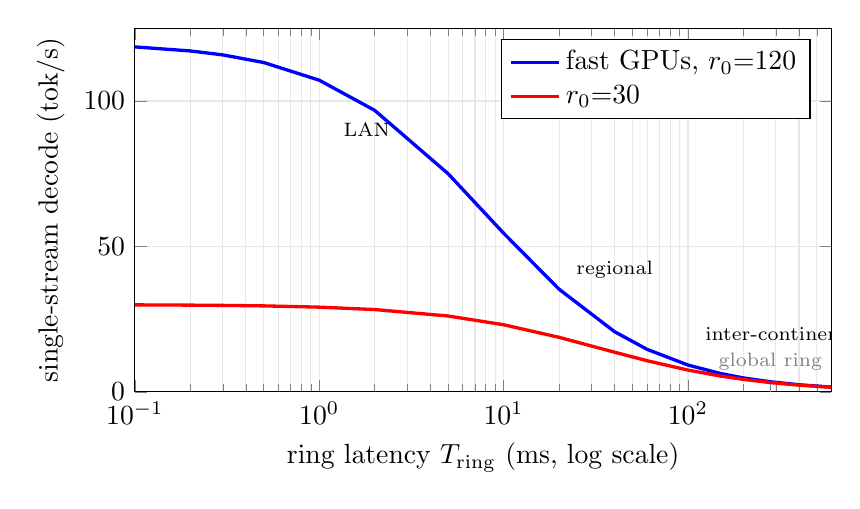
\begin{tikzpicture}
\begin{axis}[
  width=0.86\linewidth, height=6.2cm,
  xmode=log, log basis x=10,
  xlabel={ring latency $\Tring$ (ms, log scale)},
  ylabel={single-stream decode (tok/s)},
  xmin=0.1, xmax=600, ymin=0, ymax=125,
  grid=both, grid style={gray!18},
  legend pos=north east, legend cell align=left,
  every axis plot/.append style={very thick},
]
\addplot[blue] coordinates {
(0.1,118.58)(0.2,117.19)(0.3,115.83)(0.5,113.21)(1,107.14)(2,96.77)(5,75.00)(10,54.55)(20,35.29)(40,20.69)(60,14.63)(100,9.23)(150,6.32)(200,4.80)(280,3.47)(400,2.45)(600,1.64)};
\addlegendentry{fast GPUs, $r_0{=}120$}
\addplot[red] coordinates {
(0.1,29.91)(0.2,29.82)(0.3,29.73)(0.5,29.56)(1,29.13)(2,28.30)(5,26.09)(10,23.08)(20,18.75)(40,13.64)(60,10.71)(100,7.50)(150,5.45)(200,4.29)(280,3.19)(400,2.31)(600,1.58)};
\addlegendentry{$r_0{=}30$}
\draw[dashed,gray] (axis cs:280,0) -- (axis cs:280,3.47);
\node[anchor=south,font=\scriptsize,gray] at (axis cs:280,3.9) {global ring};
\node[anchor=west,font=\scriptsize] at (axis cs:1.2,90) {LAN};
\node[anchor=west,font=\scriptsize] at (axis cs:22,42) {regional};
\node[anchor=west,font=\scriptsize] at (axis cs:110,20) {inter-continental};
\end{axis}
\end{tikzpicture}
\caption{The wall. Two accelerator ceilings, $r_0=30$ and $r_0=120$\,tok/s, collapse onto the
\emph{same} curve as $\Tring$ grows: past $\sim$100\,ms the two are within $\sim$2\,tok/s. Beyond a
few tens of milliseconds of ring latency, single-stream decode is set by the network, not the GPU.
Analytical ($r=1/(C+\Tring)$).}
\label{fig:wall}
\end{figure}

\paragraph{The GPU stops mattering.} The most important reading of Figure~\ref{fig:wall} is the
convergence of the two curves. Hold $\Tring=280$\,ms and vary the local ceiling: $r_0=15\to
2.9$, $30\to3.2$, $60\to3.4$, $120\to3.5$, $1000\to3.6$\,tok/s. A $67\times$ faster accelerator buys
a $1.2\times$ faster stream. Once the ring is long, $r\to 1/\Tring$ and the accelerator is a rounding
error. Buying H100s to serve one interactive user over a global ring is spending on the wrong axis.

\paragraph{Why it is \emph{physics}.} $\Tring$ has a hard floor: light in fiber travels at
$c/n\approx2.04\times10^{5}$\,km/s ($n\approx1.47$), i.e.\ $\approx4.9\,\mu$s/km one-way, so a
real (non-geodesic) route accrues $\gtrsim5$--$7$\,ms per 1000\,km. Hong Kong to New York is
$\sim$13{,}000\,km great-circle; no switch, protocol, or budget reduces that hop below $\sim$110\,ms
one-way. The 130/40/110\,ms legs of our example ring are representative real fiber latencies, and
they are irreducible. This is the sense in which the title is literal: the wall is a property of
space and light, and the systems question is not how to break it but how to \emph{stop paying it
per token} --- which is Section~\ref{sec:spec}.

\section{``BitTorrent for AI'' is half-right}
\label{sec:bittorrent}

The appeal of swarm inference --- Petals-style pooling of volunteer GPUs across the internet ---
rests on an analogy to BitTorrent~\cite{petals}. The analogy is exact where it applies and
misleading where it does not, and the dividing line is precisely Section~\ref{sec:dichotomy}'s.

BitTorrent is fast because a file's chunks are \emph{independent}. A peer fetches them in any order,
from many sources at once; a high-latency peer just means a given chunk lands a little later, never
that another chunk waits. File download is throughput-bound and latency-insensitive --- the ideal
case for pooling far-flung capacity. \textbf{Everything about serving a distributed model that is
throughput-bound inherits this good behaviour}: shipping the weights to the nodes, prefilling a long
prompt, and running a large batch of independent requests (Section~\ref{sec:regimes}). For these, a
geographically spread swarm is genuinely attractive.

Single-stream decode is the opposite object. Its ``chunks'' --- the per-token forward passes --- are
\emph{maximally dependent}: each is the input to the next. There is no order but the one order, no
parallel sources, nothing to overlap the latency against. Pooling distant GPUs does not add
throughput to one stream; it lengthens the dependency chain by the distance between the pools. The
BitTorrent intuition, applied here, predicts the exact opposite of what happens. So the slogan is
half-right: \textbf{BitTorrent for AI works for weight distribution, prefill, and batched
throughput, and breaks for interactive single-stream latency} --- and it breaks hardest precisely
where users feel it, in the token-by-token cadence of a chat.

\section{The regime map: where geo-distribution wins}
\label{sec:regimes}

The same 280\,ms ring is cheap or catastrophic depending on how many tokens amortize it.

\paragraph{Prefill / TTFT amortizes the traversal over the whole prompt.} A prompt of $P$ tokens
goes through the pipeline in \emph{one} pass. The ring latency is paid once, not per token:
\begin{equation}
T_{\mathrm{TTFT}} \approx C_{\mathrm{prefill}}(P) + \Tring .
\label{eq:ttft}
\end{equation}
For a 2000-token prompt whose prefill compute is $\sim$1--2\,s on a big model, a $+$280\,ms ring is a
15--30\% tax on time-to-first-token --- noticeable, not fatal. Per prompt-token the traversal is
$280\,\text{ms}/2000\approx0.14$\,ms: amortized to nothing. Prefill is throughput-bound (Section~
\ref{sec:bittorrent}); a geo ring is fine for it.

\paragraph{Batched throughput fills the pipe.} With continuous batching, $N$ pipeline stages run on
$N$ different requests at once. Each \emph{individual} stream still crawls at
Eq.~\eqref{eq:wall}'s $r=1/(C+\Tring)$, but the \emph{aggregate} scales with pipeline depth toward
$\approx N\!\cdot\!(\text{per-stage rate})$ until a stage saturates. This is the BitTorrent regime
done right: many independent streams are the independent chunks that keep the pipe full. High
aggregate tok/s, high per-stream latency --- excellent for offline/batch, useless as a proxy for one
user's experience.

\begin{table}[h]
\centering
\small
\caption{The regime map. Geo-distribution is bandwidth-cheap everywhere; it is latency-cheap only
where many tokens share one traversal.}
\label{tab:regime}
\begin{tabular}{l l l l}
\toprule
Workload & Bound by & Geo ring 280\,ms? & Why\\
\midrule
Weight distribution      & throughput & \textbf{great}     & independent chunks (BitTorrent)\\
Prefill / TTFT           & throughput & \textbf{fine}      & one traversal per prompt (Eq.~\ref{eq:ttft})\\
Batched serving (aggregate) & throughput & \textbf{great}  & depth fills the pipe, $\sim\!N\times$\\
\textbf{Single-stream decode} & \textbf{dependency} & \textbf{hard} & one traversal \emph{per token} (Eq.~\ref{eq:wall})\\
\bottomrule
\end{tabular}
\end{table}

The map (Table~\ref{tab:regime}) is the practical statement of the thesis: only the bottom row is
hard, and it is hard because it is the only dependency-bound row. The next section attacks exactly
that row.

\section{The cure: speculative decoding amortizes the traversal}
\label{sec:spec}

The wall is that decode pays $\Tring$ \emph{per token}. Speculative decoding~\cite{leviathan,chen}
changes the denominator: it makes the network pay $\Tring$ \emph{per round}, where a round produces
several tokens. It is the one lever that attacks the dependency structure itself rather than the
constants.

\paragraph{Mechanism.} A small \emph{draft} model runs \emph{locally} on the entry node --- no
network in its loop --- and autoregressively proposes $K$ candidate tokens. Those $K$ tokens are
then fed as a length-$K$ sequence to the large distributed \emph{target} model, which verifies them
in a \emph{single} pipeline pass, prefill-style: the $K$ candidates flow through the ring together,
one traversal, not $K$. The target accepts the longest correct prefix under the standard
speculative-sampling rule (which preserves the target's exact output distribution) and corrects the
first mismatch. The expensive thing --- the trip around the ring --- happens once per round instead
of once per token.

\paragraph{Expected tokens per round.} Let each draft token be accepted independently with
probability $\alpha$ (the empirical acceptance rate). The number of accepted drafts $A$ satisfies
$\Pr[A\ge j]=\alpha^{j}$ for $j\le K$, so
$\mathbb{E}[A]=\sum_{j=1}^{K}\alpha^{j}=\alpha\frac{1-\alpha^{K}}{1-\alpha}$. The target always
contributes one further token (the correction on the first reject, or a bonus token if all $K$ are
accepted), giving the closed form of Leviathan et al.~\cite{leviathan}:
\begin{equation}
\Gam(\alpha,K)\;=\;1+\mathbb{E}[A]\;=\;\frac{1-\alpha^{K+1}}{1-\alpha}
\qquad\text{expected tokens per round.}
\label{eq:gamma}
\end{equation}

\paragraph{Effective rate.} A round costs one local draft of $K$ tokens plus one target
verification pass (one traversal of the ring):
\begin{equation}
T_{\mathrm{round}} \;=\; \underbrace{K\,c_d}_{\text{local draft}}
\;+\; \underbrace{C_{\mathrm{verify}}(K) + \Tring}_{\text{one target traversal}},
\qquad
r_{\mathrm{spec}}(\alpha,K)\;=\;\frac{\Gam(\alpha,K)}{T_{\mathrm{round}}}.
\label{eq:rspec}
\end{equation}
In the memory-bandwidth-bound decode regime, verifying $K\!\le\!16$ tokens streams the weights the
\emph{same} once as a single decode step, so $C_{\mathrm{verify}}(K)\approx C$ --- the reason
speculation is nearly free on the compute side.\footnote{For large $K$ the verify pass eventually
becomes compute-bound (prefill-like) and $C_{\mathrm{verify}}(K)$ grows with $K$; that is one of the
two forces creating an optimal $K$ below, the other being the geometric decay $\alpha^{K}$ of the
marginal acceptance. We take $C_{\mathrm{verify}}\!\approx\!C$ over the plotted range $K\le24$, which
is accurate for a 700B-class model where 24 tokens is still far below the arithmetic-intensity
knee.} Substituting the closed form,
\begin{equation}
\boxed{\;
r_{\mathrm{spec}}(\alpha,K)\;=\;\frac{1}{\,K\,c_d + C + \Tring\,}\cdot\frac{1-\alpha^{K+1}}{1-\alpha}
\;}
\label{eq:boxed}
\end{equation}
The structure is the whole point: $\Tring$ sits in the denominator once, divided into by
$\Gam(\alpha,K)$ tokens. The effective per-token network cost falls from $\Tring$ to
$\Tring/\Gam(\alpha,K)$.

\paragraph{Numbers on the global ring.} Take the intercontinental $\Tring=280$\,ms, target
$C=33$\,ms, and a fast local draft $c_d=5$\,ms ($r_d=200$\,tok/s). Baseline single-stream decode is
$1/(0.033+0.280)=3.2$\,tok/s. Table~\ref{tab:spec} and Figure~\ref{fig:spec} evaluate
Eq.~\eqref{eq:boxed}.

\begin{table}[h]
\centering
\small
\caption{Speculative decode on the 280\,ms global ring, from Eq.~\eqref{eq:boxed}
($C{=}33$\,ms, $c_d{=}5$\,ms). $\Gam$ = expected tokens/round; $r$ = effective tok/s.
Baseline (no speculation) $=3.2$\,tok/s. Analytical.}
\label{tab:spec}
\begin{tabular}{c cc cc cc c}
\toprule
& \multicolumn{2}{c}{$K=4$} & \multicolumn{2}{c}{$K=8$} & \multicolumn{2}{c}{$K=16$} & best\\
\cmidrule(lr){2-3}\cmidrule(lr){4-5}\cmidrule(lr){6-7}
$\alpha$ & $\Gam$ & $r$ & $\Gam$ & $r$ & $\Gam$ & $r$ & tok/s ($K^{\star}$)\\
\midrule
0.6 & 2.31 & 6.9 & 2.47 & 7.0 & 2.50 & 6.4 & 7.1 ($K{=}6$)\\
0.7 & 2.77 & 8.3 & 3.20 & 9.1 & 3.33 & 8.5 & 9.1 ($K{=}8$)\\
0.8 & 3.36 & 10.1 & 4.33 & 12.3 & 4.89 & 12.4 & 12.7 ($K{=}12$)\\
0.9 & 4.10 & 12.3 & 6.13 & 17.3 & 8.33 & 21.2 & 21.6 ($K{=}21$)\\
\bottomrule
\end{tabular}
\end{table}

\begin{figure}[h]
\centering
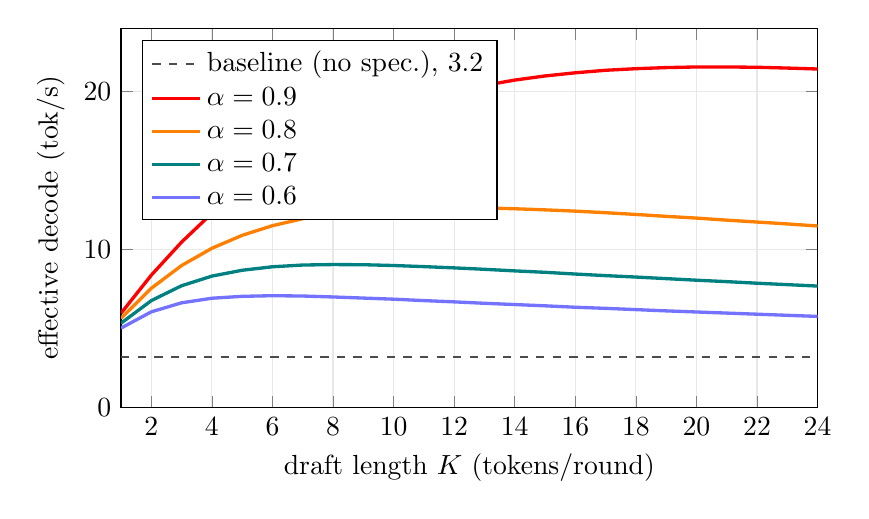
\begin{tikzpicture}
\begin{axis}[
  width=0.86\linewidth, height=6.4cm,
  xlabel={draft length $K$ (tokens/round)},
  ylabel={effective decode (tok/s)},
  xmin=1, xmax=24, ymin=0, ymax=24,
  grid=both, grid style={gray!18},
  legend pos=north west, legend cell align=left,
  every axis plot/.append style={very thick},
]
\addplot[black!70,dashed,thick] coordinates {(1,3.19)(24,3.19)};
\addlegendentry{baseline (no spec.), 3.2}
\addplot[red] coordinates {(1,5.97)(2,8.38)(3,10.47)(4,12.29)(5,13.85)(6,15.20)(7,16.35)(8,17.34)(9,18.18)(10,18.89)(11,19.48)(12,19.98)(13,20.38)(14,20.72)(15,20.98)(16,21.18)(17,21.34)(18,21.44)(19,21.51)(20,21.55)(21,21.55)(22,21.53)(23,21.48)(24,21.42)};
\addlegendentry{$\alpha=0.9$}
\addplot[orange] coordinates {(1,5.65)(2,7.55)(3,8.99)(4,10.08)(5,10.90)(6,11.51)(7,11.95)(8,12.25)(9,12.46)(10,12.58)(11,12.64)(12,12.66)(13,12.63)(14,12.58)(15,12.51)(16,12.43)(17,12.33)(18,12.22)(19,12.10)(20,11.99)(21,11.86)(22,11.74)(23,11.62)(24,11.49)};
\addlegendentry{$\alpha=0.8$}
\addplot[teal] coordinates {(1,5.34)(2,6.77)(3,7.71)(4,8.32)(5,8.69)(6,8.91)(7,9.02)(8,9.05)(9,9.04)(10,8.99)(11,8.92)(12,8.84)(13,8.75)(14,8.65)(15,8.56)(16,8.45)(17,8.35)(18,8.26)(19,8.16)(20,8.06)(21,7.97)(22,7.87)(23,7.78)(24,7.69)};
\addlegendentry{$\alpha=0.7$}
\addplot[blue!55] coordinates {(1,5.03)(2,6.06)(3,6.63)(4,6.92)(5,7.04)(6,7.08)(7,7.06)(8,7.00)(9,6.93)(10,6.86)(11,6.77)(12,6.69)(13,6.60)(14,6.52)(15,6.44)(16,6.35)(17,6.28)(18,6.20)(19,6.12)(20,6.05)(21,5.98)(22,5.91)(23,5.84)(24,5.77)};
\addlegendentry{$\alpha=0.6$}
\end{axis}
\end{tikzpicture}
\caption{The cure. Effective single-stream decode on the \emph{same} 280\,ms global ring, from
Eq.~\eqref{eq:boxed}. Speculation lifts the 3.2\,tok/s baseline (dashed) to 7--21\,tok/s. Each curve
has an optimum $K$: too small wastes the traversal, too large is drowned by the geometric decay
$\alpha^K$ and the growing draft cost $Kc_d$. Higher acceptance $\alpha$ both raises the ceiling and
pushes $K^{\star}$ out. Analytical.}
\label{fig:spec}
\end{figure}

\paragraph{Reading the result.} On a ring that floors naive decode at 3.2\,tok/s, a draft with
acceptance $\alpha=0.8$ recovers $\sim$12.7\,tok/s ($4.0\times$) and $\alpha=0.9$ recovers
$\sim$21.6\,tok/s ($6.8\times$) --- from a bad slideshow to a readable stream, on the identical
intercontinental deployment, with no faster hardware and no shorter cable. The mechanism is not a
constant-factor tuning; it is a change in what the network is charged for. Naive decode pays one
traversal per emitted token; speculation pays one traversal per $\Gam(\alpha,K)$ emitted tokens, and
$\Gam$ is exactly the knob acceptance gives you. This is why speculative decoding is \emph{the}
lever for interactive geo-distributed serving, not one option among several: it is the only cure
that divides the wall instead of chipping at it.

\paragraph{The optimum is real and worth hitting.} Each curve in Figure~\ref{fig:spec} peaks. Below
$K^{\star}$ the fixed $\Tring$ is shared over too few tokens; above it, marginal drafts are accepted
with probability $\alpha^{K}\!\to\!0$ while still costing draft time $c_d$ and, eventually, verify
compute. The peak drifts right with $\alpha$ ($K^{\star}\!:\,6\to8\to12\to21$ for
$\alpha=0.6\to0.9$) because a better draft keeps paying off for longer. A deployment should tune $K$
to its measured acceptance and ring, not to a fixed default --- the difference between $K{=}4$ and
$K^{\star}$ is $\sim$1.7$\times$ at $\alpha=0.9$.

\section{Placement laws}
\label{sec:placement}

Four heuristics fall directly out of the models above; the first two are strategy, the last two are
free.

\begin{enumerate}[leftmargin=1.5em,itemsep=3pt]
\item \textbf{Regional-first placement.} $\Tring$ dominates $r$ (Eq.~\ref{eq:wall}), so pack the
whole pipeline into one region before spanning regions. A same-metro ring ($\Tring\!\approx\!2$\,ms)
is 94\% of local; a global ring is 11\%. Span a WAN only when memory capacity forces it, and when you
do, expect to pay for speculation (Section~\ref{sec:spec}) to stay interactive. LAN neighbours are
near-native; distant neighbours are a different regime.
\item \textbf{Speculate across every slow boundary.} Any ring above a few tens of milliseconds
should run a local draft. It is the only lever that touches the $\Tring$-per-token term, and it
composes with placement: regional-first shortens $\Tring$, speculation amortizes whatever remains.
\item \textbf{Co-locate embed $+$ first layers $+$ head $+$ sampler on the entry node} (free). Makes
the sample$\to$embed turnaround local and closes the ring in exactly $N$ hops instead of $N{+}1$
(Section~\ref{sec:wall}). One node owns both ends.
\item \textbf{Keep the KV cache local to each node's layers} (free, and automatic in PP). The KV
cache never crosses the wire; only the 32\,KiB hidden state does (Section~\ref{sec:bandwidth}). Do
nothing that would ship KV state between nodes per step --- it is the large state, and it has no
reason to move.
\end{enumerate}

\section{Why pipeline-, not tensor-, parallel over slow links}
\label{sec:pptp}

The choice of \emph{how} to split the model is not free, and over a WAN it is decisive. The two
options generate fundamentally different network traffic per token.

\textbf{Pipeline parallel (PP)} splits by layer. Per token, the hidden state crosses each node
boundary once: $N$ point-to-point hops on the critical path, each moving the 32\,KiB of
Eq.~\eqref{eq:bhop}. Critical-path network latency per token $=\Tring=\sum_{i=1}^N\ell_i$.

\textbf{Tensor parallel (TP)} splits each layer's matrices across nodes~\cite{megatron}. Every layer
must \emph{all-reduce} partial results across all $N$ nodes to reconstruct the activation --- roughly
two collectives per layer (one after attention, one after the MLP). That is $\sim\!2L$ global
synchronizations per token, each of which, even counted optimistically as a single round-trip
($\ge\!2\bar\ell$; a ring all-reduce is worse, $2(N{-}1)$ serial steps), puts a barrier on the
critical path. Critical-path network latency per token $\gtrsim 2L\cdot2\bar\ell=4L\bar\ell$.

\paragraph{The traffic law.} Comparing the two, with $\bar\ell$ the mean one-way hop and
$\Tring\approx N\bar\ell$:
\begin{equation}
\frac{(\text{TP latency/token})}{(\text{PP latency/token})}
\;\gtrsim\;\frac{4L\bar\ell}{N\bar\ell}\;=\;\frac{4L}{N}.
\label{eq:pptp}
\end{equation}
\textbf{PP costs $O(\text{nodes})$ hops per token; TP costs $O(\text{layers})$ collectives per
token.} Since a model always has far more layers than nodes ($L\gg N$) and each TP collective is a
global barrier rather than a single hand-off, PP wins by a wide, structural margin: for $L=100$,
$N=3$, Eq.~\eqref{eq:pptp} gives $\gtrsim\!130\times$ less critical-path latency, and it is a lower
bound (a realistic ring all-reduce adds another $\sim(N{-}1)$ factor). TP also moves more bytes
($\sim\!2\dmodel b$ per node per collective, $\times 2L$), but latency alone settles it. TP belongs
\emph{inside} a node or an NVLink domain, where $\bar\ell$ is nanoseconds; across any link where
$\bar\ell$ is milliseconds, TP multiplies the wall by $\sim\!4L/N$ and PP is the only sane topology.
This is the structural companion to Section~\ref{sec:bandwidth}: PP's crossing tensor is
depth-independent precisely because it hands off once per node, and that is the same property that
makes it latency-cheap.

\section{What this paper claims, and what it does not}
\label{sec:honesty}

This is an analysis paper, and the analytical models \emph{are} the contribution --- so the line
between derived and measured is drawn explicitly.

\textbf{Measured (one number).} The 280\,MB/s link goodput is real: iperf3 over a direct 2.5\,GbE
cable on our mesh, sustained TCP ($\approx$2.24\,Gbit/s). It anchors the bandwidth claim in
Section~\ref{sec:bandwidth} and nothing else.

\textbf{Physical (not our measurement).} The one-way fiber latencies (40--130\,ms legs, 280\,ms
ring) are representative of real intercontinental routes and are bounded below by the speed of light
in fiber ($\approx$4.9\,$\mu$s/km). We cite the floor, not a traceroute we ran.

\textbf{Parameters (stated, not claimed).} $r_0=30$\,tok/s, $r_d=200$\,tok/s, $\alpha\in[0.6,0.9]$,
$\dmodel=16384$, $L\approx100$. These are reference values chosen to be representative of a
700B-class model with a small local draft; every table and plot is a closed-form evaluation at these
values, and the \emph{shape} of every result (the $1/(C+\Tring)$ wall, the $\Tring/\Gam$
amortization, the $4L/N$ law) is independent of the specific numbers.

\textbf{Not claimed.} We report no end-to-end wall-clock from a running geo-distributed deployment;
no measured acceptance rates for a specific draft/target pair; no serving-throughput sweep; no
overlap/async-speculation optimizations (which only improve the cure). Real acceptance depends on
the draft, the target, and the prompt distribution, and real rings have jitter and packet loss the
constant-$\ell$ model omits. The models predict \emph{regimes and ratios}, and those are what the
paper stands behind.

\section{Conclusion}
\label{sec:conclusion}

Distributing a large language model across machines is bandwidth-cheap and latency-expensive, and
the two costs live in different regimes. Bandwidth is trivial because the only tensor crossing a
pipeline boundary is a $\sim$32\,KiB hidden state --- depth-independent, KV-cache-free,
$\sim$0.1\,ms on a commodity link. Latency is a wall because autoregressive decode is a strict
dependency chain: every token traverses every node, the next cannot start until this one returns,
and so single-stream decode is floored at $1/(C+\Tring)$ --- $\approx$3\,tok/s on a global ring,
\emph{independent of the accelerator}, because the wall is the speed of light in fiber. The
``BitTorrent for AI'' picture is right for the throughput-bound work (weights, prefill, batch) and
wrong for the one dependency-bound workload (interactive decode) --- and that is the only workload
that is hard. The cure is to change what the network is charged for: speculative decoding turns $K$
sequential traversals into one, dividing the wall by the accepted-tokens-per-round $\Gam(\alpha,K)$
and recovering 12--21\,tok/s on the identical 280\,ms ring. Combined with regional-first placement, a
co-located ring turn, node-local KV, and pipeline- (never tensor-) parallelism over the slow links,
geo-distributed inference is not a contradiction --- it is a latency-engineering problem with a known
solution. The physics sets the floor; speculation decides how often you pay it.

\begin{thebibliography}{9}
\small
\bibitem{leviathan} Y.~Leviathan, M.~Kalman, Y.~Matias.
\emph{Fast Inference from Transformers via Speculative Decoding.} ICML 2023.
\bibitem{chen} C.~Chen, S.~Borgeaud, G.~Irving, J.-B.~Lespiau, L.~Sifre, J.~Jumper.
\emph{Accelerating Large Language Model Decoding with Speculative Sampling.} arXiv:2302.01318, 2023.
\bibitem{petals} A.~Borzunov, D.~Baranchuk, T.~Dettmers, M.~Ryabinin, et al.
\emph{Petals: Collaborative Inference and Fine-tuning of Large Models.} ACL 2023 (System Demonstrations).
\bibitem{gpipe} Y.~Huang, Y.~Cheng, A.~Bapna, et al.
\emph{GPipe: Efficient Training of Giant Neural Networks using Pipeline Parallelism.} NeurIPS 2019.
\bibitem{megatron} M.~Shoeybi, M.~Patwary, R.~Puri, P.~LeGresley, J.~Casper, B.~Catanzaro.
\emph{Megatron-LM: Training Multi-Billion Parameter Language Models Using Model Parallelism.}
arXiv:1909.08053, 2019.
\bibitem{pipedream} D.~Narayanan, A.~Harlap, A.~Phanishayee, et al.
\emph{PipeDream: Generalized Pipeline Parallelism for DNN Training.} SOSP 2019.
\bibitem{xbackend} Hanzo AI. \emph{Edge LLM Inference Across Commodity Accelerators: hanzo-engine at
llama.cpp Decode Parity on Every Backend.} hanzo-engine white paper (companion, measured).
\end{thebibliography}

\end{document}
